\documentclass[aspectratio=169]{beamer}
\usetheme{A}

\usepackage{stmaryrd}
\usepackage{fontspec}
\usepackage{unicode-math}
\setmainfont{Libertinus Serif}
\setsansfont{Libertinus Sans}
\setmonofont{Libertinus Mono}
\setmathfont{Libertinus Math}

\usepackage{xcolor}
\usepackage{tabularx}
\usepackage{booktabs}
\usepackage{multirow}

\usepackage{proof}
\usepackage{eqparbox}

\usepackage[normalem]{ulem}

\usepackage{tikz}
\usetikzlibrary{decorations.pathreplacing, calc, fit, positioning}
\usepackage{tikz-qtree}
\tikzset{
	unary/.style={thin,double},
	head/.style={ultra thick}
}
\newcommand{\tikzmark}[2]{%
    \tikz[remember picture,overlay] \coordinate (tikzmark-#1-start) at (0,0);%
    {#2}%
    \tikz[remember picture,overlay] \coordinate (tikzmark-#1-end) at (0,0);%
    \tikz[remember picture,overlay] \node[anchor=center, outer sep=0pt] (#1) at ($ (tikzmark-#1-start)!0.5!(tikzmark-#1-end) $) {\vphantom{#2}};%
}
\newcommand{\markproofleaf}[2]{\tikzmark{#1}{\textcolor{textcolor}{#2}}}
\newcommand{\arc}[5][0]{%
	\draw[->] (#2) .. controls
      ($(#2)!0.33!(#3) + (0,#4)$) and
      ($(#3)!0.33!(#2) + (0,#4)$)
    .. node[below] {#5} ($(#3.center) + (#1, -3pt)$);
}


\usepackage{relsize}
\usepackage{enumitem}
\setlist[itemize]{label=\textcolor{pred}{$\bullet$}, topsep=0pt, itemsep=0pt}
\setlist[itemize,2]{label=\textcolor{pred}{$\circ$}, topsep=0pt, itemsep=0pt,leftmargin=1.5em}

\definecolor{light}{rgb}{0.38,0.38,0.38}
\newcommand{\light}[1]{\textcolor{light}{#1}}
\newcommand{\rulestyle}[1]{#1}
\newcommand{\Ax}{\rulestyle{Ax}}
\newcommand{\EX}{\rulestyle{Ex}}
\newcommand{\li}{\to}
\newcommand{\bs}{\backslash}
\newcommand{\ty}[1]{#1}
\newcommand{\te}[1]{#1}
\newcommand{\appr}{\triangleright}
\newcommand{\appl}{\triangleleft}
\newcommand{\lambdar}{\lambda^r}
\newcommand{\lambdal}{\lambda^l}
\renewcommand{\otimes}{⊗}
\newcommand{\crossmark}{✘}
\newcolumntype{C}{>{\centering\arraybackslash}X}
\newcommand{\alertat}[2]{\alt<#1>{\alert{#2}}{#2}}

\newcommand{\colorat}[3]{\alt<#2>{\textcolor{#1}{#3}}{#3}}
\newcommand{\lightat}[2]{\colorat{light}{#1}{#2}}
\newcommand{\showat}[2]{\alt<#1>{#2}{}}
\newcommand{\strat}[2]{\alt<#1>{\sout{#2}}{#2}}
\newcommand{\caseof}[3]{\text{case }{\te{#1}}\text{ of }{\te{#2}}\text{ in }{\te{#3}}}
\renewcommand{\emptyset}{()}
\newcommand{\inferat}[4][]{%
	\alt<#2>{
		\infer[#1]{#3}{#4}
	}{%
		\deduce[\visible<#2>{#1}]{\visible<#2>{#3}}{#4}
	}%
}
\newcommand{\infereat}[4][]{%
	\alt<#2>{
		\infer=[#1]{#3}{#4}
	}{%
		\deduce[\visible<#2>{#1}]{\visible<#2>{#3}}{#4\vspace{2pt}}
	}%
}
\newcommand{\subst}[1]{\llbracket{#1}\rrbracket}
\newcommand{\struct}[2][]{\langle #2 \rangle^{\scalebox{0.66}{\dep{#1}}}}
\newcommand{\alertstruct}[2][]{\textcolor{pred}{\langle} #2 \textcolor{pred}{\rangle}}
\renewcommand{\alert}[1]{\textcolor{pred}{#1}}
\newcommand{\Lex}{\rulestyle{Lex}}
\newcommand{\w}[1]{\text{#1}}
\newcommand{\sbr}{\mathbin{\cdot}}
\newcommand{\Ass}{\rulestyle{A}}
\newcommand{\Prim}[1][]{\ensuremath{{\mathsf{Prim}_{#1}}}}
\newcommand{\Cons}[1][]{\ensuremath{{\mathsf{Cons}_{#1}}}}
\newcommand{\types}{\ensuremath{\mathcal{U}}}
\newcommand{\terms}{\ensuremath{\Lambda}}

\makeatletter
\newcommand{\getfontdim}[1]{%
  \fontdimen22
  \ifx#1\displaystyle\textfont\else
  \ifx#1\textstyle\textfont\else
  \ifx#1\scriptstyle\scriptfont\else
  \scriptscriptfont\fi\fi\fi 2
}
\makeatother

% ratio: 1.8/2.75
\newcommand{\domodaldiamondscale}[2]{\raisebox{0.175\getfontdim{#1}}{\scalebox{1.1}{\ensuremath{#1#2}}}}
\newcommand{\domodalboxscale}[2]{\raisebox{0.15\getfontdim{#1}}{\scalebox{0.85}{\ensuremath{#1#2}}}}
\newcommand{\dmodaldiamondscale}[1]{\mathpalette\domodaldiamondscale{#1}\relax}
\newcommand{\dmodalboxscale}[1]{\mathpalette\domodalboxscale{#1}\relax}
\newcommand{\domodalxdiascale}[2]{\raisebox{0.175\getfontdim{#1}}{\scalebox{1.1}{\ensuremath{#1#2}}}}
\newcommand{\modalxdiascale}[1]{\mathpalette\domodalxdiascale{#1}\relax}
\newcommand{\modalboxscale}[1]{\mathpalette\domodalboxscale{#1}\relax}
\renewcommand{\diamond}{\dmodaldiamondscale{\diamondsuit}}
\newcommand{\bx}{\dmodalboxscale{\Box}}
\newcommand{\xdiamond}{\modalxdiascale{\vardiamondsuit}}
\newcommand{\xbx}{\modalboxscale{\blacksquare}}
\newcommand{\dep}[1]{\ensuremath{\mathsf{#1}}}
\newcommand{\deps}{\mathrm{D}}
\newcommand{\adjuncts}{\mathrm{A}}
\newcommand{\complements}{\mathrm{C}}
\newcommand{\ddia}[1][]{\diamond^{\scalebox{0.66}{\dep{\smaller{#1}}}}}
\newcommand{\dbox}[1][]{\bx^{\scalebox{0.66}{\dep{\smaller{#1}}}}}
\newcommand{\dxbox}[1][]{\xbx^{\scalebox{0.66}{\dep{\smaller{#1}}}}}
\newcommand{\dxdia}[1][]{\xdiamond^{\scalebox{0.66}{\dep{\smaller{#1}}}}}


\newcommand{\su}{\dep{su}}
\newcommand{\obj}{\dep{obj1}}
\newcommand{\io}{\dep{obj2}}
\newcommand{\ddet}{\dep{det}}
\newcommand{\dmod}{\dep{mod}}
\newcommand{\predc}{\dep{predc}}
\newcommand{\body}{\dep{body}}

\makeatletter
\newcommand{\domodaltermscale}[2]{\raisebox{0.25\getfontdim{#1}}{\scalebox{0.85}{\ensuremath{#1#2}}}}
\makeatother
\newcommand{\dmodaltermscale}[1]{\mathpalette\domodaltermscale{#1}\relax}
\newcommand{\boxelim}{\dmodaltermscale{▼}}
\newcommand{\boxintro}{\dmodaltermscale{▲}}
\newcommand{\diaelim}{\dmodaltermscale{▽}}
\newcommand{\diaintro}{\dmodaltermscale{△}}
\newcommand{\dboxelim}[1][]{\boxelim^{\dep{#1}}}
\newcommand{\ddiaelim}[1][]{\diaelim^{\dep{#1}}}
\newcommand{\ddiaintro}[1][]{\diaintro^{\dep{#1}}}
\newcommand{\dboxintro}[1][]{\boxintro^{\dep{#1}}}


\title{Grammaticality as Provability}
\date{%
	\\
	Groningen Logic Seminar\\
	May 2025
	\vspace{6em}
}
\author{\light{Konstantinos Kogkalidis}}
\renewcommand{\arraystretch}{1.15}


\begin{document}

\maketitle

\begin{frame}{The Big Picture}
	\smaller
	
	\begin{minipage}[t]{0.45\textwidth}
	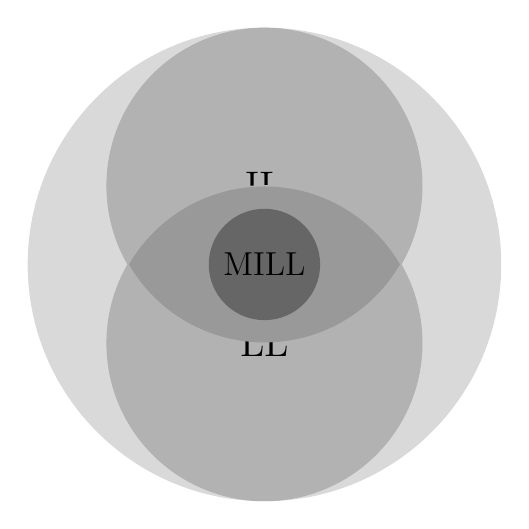
\begin{tikzpicture}[
		one/.style={fill=gray!30, draw=gray!30},
		two/.style={fill=gray!60, draw=gray!60},
		three/.style={fill=gray!80, draw=gray!80},
		four/.style={fill=black!60, draw=black!60}
		]
		\draw[one] (0,0) circle (3);
		\visible<1>{\node at (0, 0) {\Large CL};}
		\visible<2,4->{
		\draw[two] (0, 1) circle (2);
		\visible<2>{\node at (0, 1) {\Large IL};}
		}
		\visible<3,4->{
		\draw[two] (0, -1) circle (2);
		\visible<3>{\node at (0, -1) {\Large LL};}
		}
		\visible<4->{
		\clip (0, 1) circle (1.99);
		\clip (0, -1) circle (1.99);
		\draw[three] (0,0) circle (2.6);
		\visible<4>{\node at (0, 0) {\Large ILL};}
		}
		\visible<5->{
		\draw[four] (0,0) circle (0.7);
		\visible<5>{\node at (0, 0) {\large MILL};}
		}
	\end{tikzpicture}%
	\end{minipage}\hfill%
	\begin{minipage}[t]{0.55\textwidth}
	\vspace{-5cm}
	\begin{itemize}
		\item \eqmakebox[logic][l]{\alert{CL}} \light{(folklore\dots)}
		\visible<2->{
		\item \eqmakebox[logic][l]{\alert{IL}} \light{(Heyting, 1930)}\\
		{no excluded middle, no involutive negation}
		}
		\visible<3->{
		\item \eqmakebox[logic][l]{\alert{LL}} \light{(Girard, 1987)}\\
		{truth $\equiv$ resource; no weakening, no contraction}
		}
		\visible<4->{
		\item \eqmakebox[logic][l]{\alert{ILL}} \\
		{= LL $\cap$ IL}
		}
		\visible<5->{
		\item \eqmakebox[logic][l]{\alert{MILL}} \\
		{= ILL without additives}
		}
	\end{itemize}\vfill
	\end{minipage}
\end{frame}

\begin{frame}{MILL\\
\smaller\light{\quad\alt<10->{term calculus}{typing rules}}}
	\smaller
	
	\begin{minipage}{.5\textwidth}
		\begin{tabular}{@{}r@{ }l@{}}
		 	\multicolumn{2}{@{}l}{\textbf{Types}}\\
			$\ty{A, B, C}$ & $:= p \ | \ \ty{A\li B} \ | \ \ty{A\otimes B}$ \qquad \light{($p \in \Prim$)}\\
		    \addlinespace
			\multicolumn{2}{@{}l}{\uncover<2->{\textbf{Structures}}}\\
		  	\uncover<2->{
		   	$\Gamma, \Delta$ & $:= \ \emptyset \ | \ \Gamma\sbr \ty{A}$
		   	}
		\end{tabular}
	\end{minipage}
	\vspace{1em}
	
	\centering
	\begin{tabularx}{0.8\textwidth}{@{}CC@{}}
	\multicolumn{2}{@{}c@{}}{\uncover<3,9->{\alertat{3}{
		$\infer[\Ax]{\showat{10-}{\light{\te{x}} : }\ty{A} \vdash \showat{10-}{\light{\te{x}} : }\ty{A}}{}$}}}\\
	\addlinespace
	\uncover<4,9->{%
	\alertat{4}{
	$\infer[\li_E]{\Gamma\sbr \Delta \vdash \showat{10-}{\light{\te{s~t}} : }\ty{B}}{\Gamma \vdash \showat{10-}{\light{\te{s}} : }\ty{A \li B} & \Delta \vdash \showat{10-}{\light{\te{t}} : }\ty{A}}$
	}}
	&
	\uncover<5,9->{%
	\alertat{5}{
	$\infer[\li_I]{\Gamma \vdash \showat{10-}{\light{\te{\lambda x.s}} : }\ty{A \li B}}{\Gamma\sbr \showat{10}{\light{\te{x}} : }A \vdash \showat{10}{\light{\te{s}} : }B}$
	}}\\
	\addlinespace
	\uncover<7,9->{\alertat{7}{$\infer[\otimes_E]{\Gamma\sbr \Delta \vdash \showat{10-}{\light{\caseof{s}{(x, y)}{t}} : }C}{\Gamma \vdash \showat{10-}{\light{\te{s}} : }\ty{A\otimes B} & \Delta\sbr\showat{10-}{\light{\te{x}} : }\ty{A}\sbr \showat{10-}{\light{\te{y}} : }\ty{B} \vdash \showat{10-}{\light{\te{t}} : }\ty{C}}$}}
	&
	\uncover<6,9->{
	\alertat{6}{
	$\infer[\otimes_I]{\Gamma\sbr \Delta \vdash \showat{10-}{\light{\te{(x, y)}} : }\ty{A \otimes B}}{\Gamma \vdash \showat{10-}{\light{\te{x}} : }\ty{A} & \Delta \vdash \showat{10-}{\light{\te{y}} : }\ty{B}}$}}\\
	\addlinespace
	\multicolumn{2}{@{}c@{}}{
	\uncover<8->{
	\alertat{8}{
	$\infer=[\EX]{\Gamma\sbr \showat{10-}{\light{\te{y}}:}\ty{B}\sbr \showat{10-}{\light{\te{x}}:}\ty{A}\sbr \Delta \vdash \showat{10-}{\light{\te{s}}:}\ty{C}}{\Gamma\sbr \showat{10-}{\light{\te{x}}:}\ty{A}\sbr \showat{10-}{\light{\te{y}}:}\ty{B}\sbr \Delta \vdash \showat{10-}{\light{\te{s}}:}\ty{C}}$
	}}}
	\end{tabularx}
\end{frame}

\begin{frame}{Invertible Inferences}
	\smaller
	\begin{minipage}{.5\textwidth}
	\[
	\infereat{4-}{
			\ty{A_1 \otimes \dots \otimes A_n} \vdash \ty{B} 
		}{
			\infereat{3-}{
				 	\emptyset \vdash \ty{(A_1 \otimes \dots \otimes A_n)\li B}
		}{
					\infereat{2-}{
							\emptyset \vdash \ty{A_1\li \dots \li A_n\li B}
						}{
							 \Gamma_{\light{[\ty{A_1}\sbr ~\dots~ \sbr \ty{A_n}]}} \vdash \ty{B}
						}
				}
		}
	\]
	\vspace{0.5em}
	\visible<5->{
	\uncover<-6>{
	\[
		\infer=[\Gamma' \in \mathsf{S}_n(\Gamma)]{\Gamma'~ \vdash \ty{B}}{\Gamma \vdash \ty{B}}
	\]}}
	\end{minipage}
	
	\visible<6->{	
	\begin{tikzpicture}[overlay,remember picture,xshift=18em,yshift=6.5em]
	   	\draw [decoration={brace,amplitude=5pt,mirror,raise=2pt},decorate,thick,draw=pred]
    (0, -1.6) -- (0, 1.6) node[midway,right=1pt,align=left] {
    	\begin{minipage}{24em}
    	\begin{itemize}
    		\item premises are \strat{7-}{\lightat{7-}{\alertat{-6}{\textit{multisets}}}} \visible<7->{\alert{\textit{sequences}} ($n!$ as many)}
    		\item \alert{$\otimes$} and \alert{$\sbr$} are \textit{\alert{variadic}} \strat{7-}{\lightat{7-}{and \textit{\alertat{-6}{order-insensitive}}}}
    		\item[] \vdots
	    \end{itemize}    	
    	\end{minipage}
	    };
	    \visible<7->{
	    	\node[pred, very thick, scale=5.5] at (-2.2, -1.2) {$\crossmark$};
	    }
	\end{tikzpicture}
	}
\end{frame}

\begin{frame}{Going Sub\textsuperscript{(2)}structural
\\
\quad\smaller\light{A world without exchange}}
	\smaller
	\alt<2->{
		\textbf{Now}: \\
		\qquad$
			\ty{A_1 \bs (A_2 \bs B)} \mathbin{\alert{\not\equiv}} \ty{A_2 \bs (A_1 \bs B)} \mathbin{\alert{\not\equiv}} \ty{(B / A_2) / A_1} \mathbin{\alert{\not\equiv}} \ty{(B / A_1) / A_2} \mathbin{\alert{\not\equiv}} \ty{(A_1 \bs B) / A_2} \mathbin{\alert{\not\equiv}} \ty{(A_2 \bs B) / A_1}
		$
		
		\hfill \light{all these just from $\ty{A_1\li A_2\li B}$ (!)} 
		\vfill
	
		\visible<3->{
		\textbf{Yet still}: \\
		\qquad$\ty{(A_1 \bs B)/A_2} \equiv \ty{A_1 \bs (B / A_2)}$
		
		\[
			\infer={
					\alert{\Gamma \vdash \ty{(A_1 \bs B) / A_2}}
				}{
					\infer={
						\Gamma\sbr \ty{A_2} \vdash \ty{A_1 \bs B}
					}{
						\infer={
							\ty{A_1}\sbr \Gamma\sbr \ty{A_2} \vdash \ty{B}
						}{
							\infer={
								\ty{A_1}\sbr \Gamma \vdash \ty{B / A_2}
							}{
								\alert{\Gamma \vdash \ty{A_1 \bs (B / A_2)}}
							}
						}
					}
				}
		\]
	}
	}{%
		Without \EX{}, $\li$ branches into two \alert{position-refined} variants: $\alert{/}$ and $\alert{\bs}$.\\ 
		~\light{Read: 
		\begin{tabular}{r@{ -- }l}
			$\ty{B / A}$ & ``$\ty{B}$ \textit{over} $\ty{A}$''\\
			$\ty{A \bs B}$ & ``$\ty{A}$ \textit{under} $\ty{B}$''
		\end{tabular}}\vspace{1em}
	
		\begin{center}\begin{tabularx}{0.8\textwidth}{@{}CC@{}}
		$
			\infer[\bs_E]{\Gamma\sbr \Delta \vdash \light{\te{s \appr t}} : \ty{B}}{\Gamma \vdash \light{\te{s}} : \ty{\alert{A}}  & \Delta \vdash \light{\te{t}} : \ty{\alert{A} \bs B}}
		$
		&
		$
			\infer[\bs_I]{\Gamma \vdash \light{\te{\lambdal x.s}} : \ty{\alert{A} \bs B}}{\light{\te{x}}: \ty{\alert{A}}, \Gamma \vdash \ty{B}}
		$\\
		\addlinespace\addlinespace\addlinespace
		$
			\infer[/_E]{\Gamma\sbr \Delta \vdash \light{\te{s\appl t}}:\ty{B}}{\Gamma \vdash \light{\te{s}}: \ty{B / \alert{A}}  & \Delta \vdash \light{\te{t}}: \ty{\alert{A}}}
		$
		&
		$
			\infer[/_I]{\Gamma \vdash \light{\te{\lambdar x.s}}: \ty{B / \alert{A}}}{\Gamma\sbr \light{\te{x}}: \ty{\alert{A}} \vdash \light{\te{s}}: \ty{B}}
		$
		\\
		\addlinespace\addlinespace\addlinespace
		\multicolumn{2}{c}{
		$\infer[\otimes_E]{\Gamma\sbr \alert{\Delta}\sbr \alert{\Theta} \vdash \light{\caseof{s}{(x, y)}{t}} : C}{\Gamma \vdash \light{\te{s}} : \ty{A\otimes B} & \alert{\Delta}\sbr \light{\te{x}} : \ty{A}, \light{\te{y}} : \ty{B}\sbr \alert{\Theta} \vdash \light{\te{t}} : \ty{C}}$
		}
		\end{tabularx}\end{center}
	}
\end{frame}

\begin{frame}{}
	\centering
	\vfil
	\light{The (invisible) culprit?}
\end{frame}

\begin{frame}{Going Sub\textsuperscript{(2)}structural
\\
\quad\smaller\light{A world without exchange or associativity}}
\smaller
	\begin{itemize}
		\item premises become \textit{\alert{trees}} ($C_{n-1}$ as many)
		\item \alert{$\otimes$} and \alert{$,$} become \textit{\alert{binary}}
		\item[] \vdots
	\end{itemize}\vspace{2em}

	\begin{center}\begin{tabularx}{0.8\textwidth}{@{}CC@{}}
	$
		\infer[\bs_E]{\alert{(}\Gamma\mathbin{\alert{\sbr}} \Delta\alert{)} \vdash \light{\te{s \appr t}} : \ty{B}}{\Gamma \vdash \light{\te{s}} : \ty{A}  & \Delta \vdash \light{\te{t}} : \ty{A \bs B}}
	$
	&
	$
		\infer[\bs_I]{\Gamma \vdash \light{\te{\lambdal x.s}} : \ty{A \bs B}}{\alert{(}\light{\te{x}}: \ty{A}\mathbin{\alert{\sbr}} \Gamma\alert{)} \vdash \ty{B}}
	$\\
	\addlinespace\addlinespace\addlinespace
	$
		\infer[/_E]{\alert{(}\Gamma\mathbin{\alert{\sbr}} \Delta\alert{)} \vdash \light{\te{s\appl t}}:\ty{B}}{\Gamma \vdash \light{\te{s}}: \ty{B / A}  & \Delta \vdash \light{\te{t}}: \ty{A}}
	$
	&
	$
		\infer[/_I]{\Gamma \vdash \light{\te{\lambdar x.s}}: \ty{B / A}}{\alert{(}\Gamma\mathbin{\alert{\sbr}} \light{\te{x}}: \ty{A}\alert{)} \vdash \light{\te{s}}: \ty{B}}
	$
	\\
	\addlinespace\addlinespace\addlinespace
	\multicolumn{2}{c}{
	$\infer[\otimes_E]{\Delta\subst{\alert{\Gamma}} \vdash \light{\caseof{s}{(x\sbr y)}{t}} : C}{\Gamma \vdash \light{\te{s}} : \ty{A\otimes B} & \Delta\subst{\alert{(}\light{\te{x}} : \ty{A}\mathbin{\alert{\sbr}} \light{\te{y}} : \ty{B}\alert{)}} \vdash \light{\te{t}} : \ty{C}}$
	}
	\end{tabularx}\end{center}
\end{frame}

\begin{frame}{The Small Picture\\
\quad\smaller\light{An Alternative Timeline}}
	\smaller
	
	\begin{minipage}[t]{0.45\textwidth}\centering\begin{tikzpicture}[
		g/.style={outer sep=6pt, inner sep=0pt,minimum width=4pt},e/.style={thick},
		scale=1.5
	]
		\node[g] (L) 	at (0,0)			{\alertat{1}{L}};
		\visible<2->{
		\node[g] (NL)	at (2, 0)			{\alertat{2}{NL}};
		\draw[e, ->] (L) -- (NL) node[midway,above]{-asso};
		}
		\visible<3->{
		\node[g] (LP)	at (0, -1.5)		{\alertat{3}{LP}};
		\draw[e, <-] (LP) -- (L) node[midway,left]{+comm};
		}
		\visible<4->{
		\node[g] (NLP)	at (2, -1.5)		{\alertat{4}{NLP}};
		\draw[e, ->] (NL) -- (NLP) node[midway,right]{+comm};
		\draw[e, ->] (NLP) -- (LP) node[midway,below]{+asso};
		}

	\end{tikzpicture}\end{minipage}\hfill
	% (L?)
	\begin{minipage}[t]{0.55\textwidth}\vspace{-8em}\begin{itemize}
		\item \eqmakebox[logic][l]{\alert{L}} \light{(Lambek, 1958)}
		\visible<2->{
		\item \eqmakebox[logic][l]{\alert{NL}} \light{(Lambek, 1961)}
		}
		\visible<3->{
		\item \eqmakebox[logic][l]{\alert{LP}} \light{(van Benthem, 1983)}\\
		= MILL (!)
		}
		\visible<4->{
		\item \eqmakebox[logic][l]{\alert{NLP}} \light{(\textit{ditto})}
		}

	\end{itemize}\vfill\end{minipage}\vfill
	

	\visible<5->{
		\begin{center}
		\textbf{(N)L(P)}: Grammar Logics
		\end{center}\vfill
		
		\smaller
		\begin{flushright}
		\visible<6->{\light{
			\textit{%
				``Every mathematical discovery is made twice: once by a \strat{7-}{\lightat{7-}{logician}} \alt<7->{theoretical linguist}{} and once by a \strat{7-}{\lightat{7-}{computer scientist}} \alt<7->{logician}{}''\\
 -- P. Wadler \visible<7->{(retrofitted)}
 			}
		}}
		\end{flushright}
	}
\end{frame}

\begin{frame}{(N)L(P)\\
\quad\smaller\light{Executive Summary}
}\smaller\centering
	\begin{tabular}{@{}cccc@{}}
		Logic		& $\Gamma$	& Asso	& Comm\\
		\toprule
		LP			& multiset	& $✔$ 	& $✔$\\
		L			& string	& $✔$	& $\crossmark$\\
		NL			& tree		& $\crossmark$	& $\crossmark$\\
		NLP			& mobile	& $\crossmark$	& $✔$
	\end{tabular}
\end{frame}

\begin{frame}{Type-Logical Grammar 101\\
\smaller\quad\light{The idea}
}\smaller
	\begin{center}
	\begin{tabularx}{.8\textwidth}{@{}CCC@{}}
		\toprule
		\textbf{Language}			& \textbf{Logic}			& \textbf{Computation}\\
		\toprule
		grammar						& substructural logic 		& $\lambda$-calculus\\
		syntactic category			& formula					& type\\
		\alertat{2}{word}			& \alertat{2}{hypothesis}	& \alertat{2}{variable}\\
		phrasal composition 		& inference rule			& computation step\\
		grammaticality				& provability				& type inhabitation\\
		\multicolumn{3}{c}{\larger\vdots}\\
		sentence					& proof						& program\\
		parsing						& deduction					& computation
	\end{tabularx}\end{center}\vfill
	
	\visible<2->{
	\textbf{The lexicon} -- a mapping associating words and types\\
		\light{\quad $\Lex{} : \mathsf{Words}$ $\to$ $\mathcal{P}(\types)$}
	}
\end{frame}

\begin{frame}{Pipeline}
\smaller\centering
	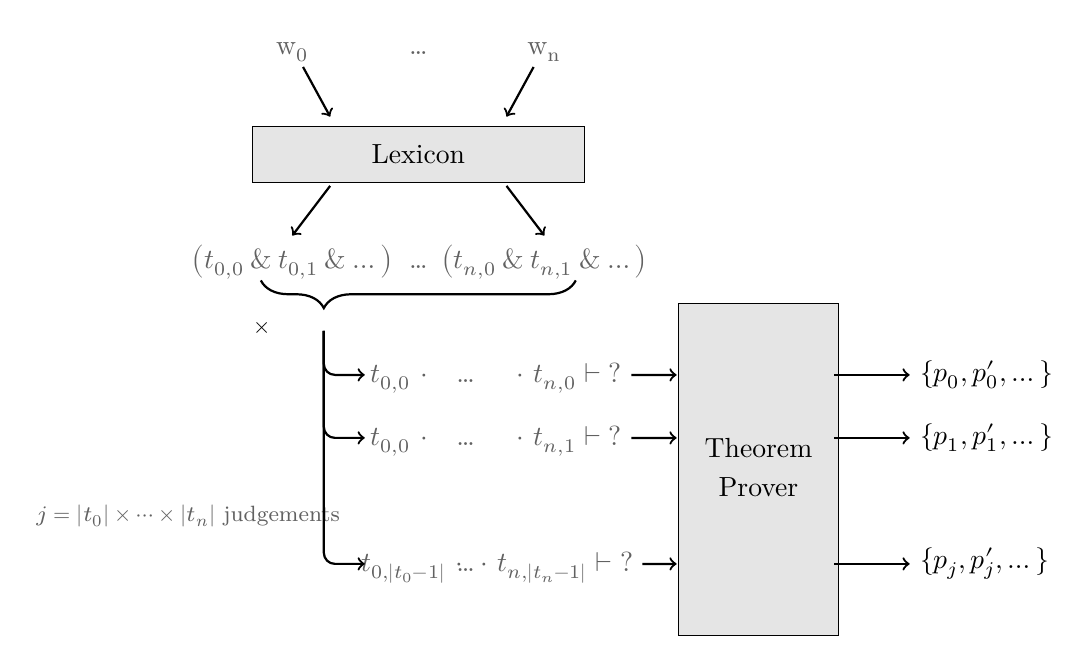
\begin{tikzpicture}[
		t/.style={text height=1.5ex, text depth=.25ex, rectangle, outer sep=0pt, color=light},
		node distance=10pt,
		arr/.style={thick,->},
		scale=0.8
	]
		\node[t] (w1) 			at (0, 0.2) {w\textsubscript{0}};
		\node[t] (wdots)		at (2, 0.2) {\dots};		
		\node[t] (wn) 			at (4, 0.2) {w\textsubscript{n}};
		\node[rectangle,draw=black, minimum width=120pt,minimum height=20pt,fill=gray!20] (lex)
							 	at (2, -1.5) {Lexicon};
		\draw[arr]  (w1) -- ++ (0.6, -1.1);
		\draw[arr] (wn) -- ++ (-0.6, -1.1);
		\node[t] (t1)			at (0, -3.2) {$\left(\ty{t}_{0,0} \mathbin{\&} \ty{t}_{0, 1} \mathbin{\&} \dots\right)$};
		\node[t] (tdots)		at (2, -3.2) 	  {\dots};
		\node[t] (tn)			at (4, -3.2) {$\left(\ty{t}_{n,0} \mathbin{\&} \ty{t}_{n,1} \mathbin{\&} \dots\right)$};
		\draw[arr] ($(w1) + (0.6, -2.2)$) -- ($(t1.north) + (0, 0.1)$);
		\draw[arr] ($(wn) + (-0.6, -2.2)$) -- ($(tn.north) + (0, 0.1)$);
		\draw [thick,decorate,decoration={brace,aspect=0.2,amplitude=10pt,mirror}] (-0.5,-3.5) -- (4.5,-3.5) 
				node[black,xshift=-113.5pt,yshift=-0.6cm] {\footnotesize $\times$}
				node[xshift=-140pt, yshift=-8.5em, align=right,color=light] {\smaller $j = |\ty{t}_0| \times \dots \times |\ty{t}_n|$ judgements};				
		\node[t] (c11)			at (1.7, -5) {$\ty{t}_{0,0} ~ \sbr$};
		\node[t] 				at (2.75, -5) {\dots};
		\node[t] (cn1)			at (4.4, -5) {$\sbr ~\ty{t}_{n,0} \vdash ?$};
		\node[t] (c12)			at (1.7, -6) {$\ty{t}_{0,0} ~ \sbr$};
		\node[t] 				at (2.75, -6) {\dots};
		\node[t] (cn2)			at (4.4, -6) {$\sbr ~\ty{t}_{n,1} \vdash ?$};
		\node[t] (vd)			at (2.75, -7) {\vdots};
		\node[t] (c1k)			at (1.9, -8) {$\ty{t}_{0,|t_0 - 1|}~\sbr$};
		\node[t] 				at (2.75, -8) {\dots};
		\node[t] (cnk)			at (4.2, -8) {$\sbr~\ty{t}_{n,|t_n - 1|} \vdash ?$};
		\draw[arr, rounded corners] (0.5, -4.3) -- ++ (0, -0.7) -- ++ (0.65, 0);
		\draw[arr, rounded corners] (0.5, -4.3) -- ++ (0, -1.7) -- ++ (0.65, 0);
		\draw[arr, rounded corners] (0.5, -4.3) -- ++ (0, -3.7) -- ++ (0.65, 0);
		\node[rectangle, draw=black, minimum height=120pt,fill=gray!20] (pr)
								at (7.4, -6.5)	{\begin{tabular}{c}Theorem\\ Prover\end{tabular}};	
		\draw[arr] (cn1) -- ++ (1.7, 0);
		\draw[arr] (cn2) -- ++ (1.7, 0);
		\draw[arr] (cnk) -- ++ (1.9, 0);
		\draw[arr] (cn1) ++ (4.2, 0) -- ++ (1.2, 0) node[right] {$\{p_0, p_0', \dots \}$};
		\draw[arr] (cn2) ++ (4.2, 0) -- ++ (1.2, 0) node[right] {$\{p_1, p_1', \dots \}$};
		\node 					at ($(vd) + (6.6, 0)$) {\vdots};
		\draw[arr] (cnk) ++ (4.4, 0) -- ++ (1.2, 0) node[right] {$\{p_j, p_j', \dots \}$};
	\end{tikzpicture}
\end{frame}


\begin{frame}{Compositionality\smaller\\
\quad\light{A Toy Example}
}\smaller
	\alt<2>{
		\visible<2->{
		\begin{center}
			Source $\Sigma$: (N)L $\xrightarrow{\makebox[0.33in]{$\langle \eta, \theta\rangle$}}$ Target T: MILL
		\end{center}
		\textbf{Base syntactic types $\Prim_\Sigma$ :} $\ty{n}$, $\ty{np}$, $\ty{s}$\\
		\textbf{Base semantic types $\Prim_T$ :} $\ty{e}$, $\ty{t}$
		\vfill
		
		\begin{minipage}[t]{0.2\textwidth}
		\begin{tabular}{@{}l@{ = }l@{}}
			\multicolumn{2}{@{}l}{$\eta_0 : \Prim_\Sigma \to \types_T$}\\
			$\eta_0 ~ \ty{np}$ & $\ty{e}$\\
			$\eta_0 ~ \ty{s}$ & $\ty{t}$\\
			$\eta_0 ~ \ty{n}$ & $\ty{e\li t}$\\		
		\end{tabular}\end{minipage}%
		\begin{minipage}[t]{0.35\textwidth}
		$\rightsquigarrow$\hspace{2em}\begin{tabular}{@{}l@{ = }l@{}}
			\multicolumn{2}{@{}l}{$\eta : \types_\Sigma \to \types_T$}\\
			$\eta ~ \ty{p}$ & $\eta_0 ~ \ty{p}$\\
			$\eta ~ (\ty{A \bs B})$ & $\eta ~ (\ty{B / A})$ = $(\eta ~ A) \li (\eta ~ B)$\\
			\multicolumn{2}{@{}l}{\hphantom{$\eta_0$}}
		\end{tabular}		
		\end{minipage}\vfill
		
		\begin{minipage}[t]{0.2\textwidth}
		\begin{tabular}{@{}l@{ = }l@{}}
			\multicolumn{2}{@{}l}{$\theta_0 : \Cons_\Sigma \to \terms_T$}\\
			\multicolumn{2}{@{}l}{\dots}\\
		\end{tabular}\end{minipage}%
		\begin{minipage}[t]{0.35\textwidth}
		$\rightsquigarrow$\hspace{2em}\begin{tabular}{@{}l@{ = }l@{}}
			\multicolumn{2}{@{}l}{$\theta : \terms_\Sigma \to \terms_T$}\\
			$\theta ~ (\te{s \appr t})$ & $\theta ~ (\te{t \appl s})$ = $(\theta~\te{s})~ (\theta~\te{t})$
		\end{tabular}		
		\end{minipage}\vfill
		}
	}{
	\begin{center}\begin{tabular}{@{}c@{\quad}c@{\quad}c@{\quad}c@{\quad}c@{}}
		\text{syntactic calculus} & $\xrightarrow{\makebox[0.33in]{$h_1$}}$ & \text{semantic calculus} & $\xrightarrow{\makebox[0.33in]{$h_2$}}$ & \text{lexical meaning}\\
				(N)L\textsuperscript{(+)} & & MILL${}^{\text{(+)}}_{\li, \otimes}$ & & FOL / IL / \dots \\ 
		\addlinespace
		\multirow{2}{*}{\textit{surface form}} & & \textit{meaning} & & \textit{meaning} \\
		& &	{\footnotesize\light{\textit{derivational}}} & & {\footnotesize\textit{\light{lexical}}}
	\end{tabular}\end{center}\vfill
	
	$h_i := \langle \eta_i, \theta_i \rangle$, where:
	\begin{itemize}
		\item $\eta$ an action on types
		\item $\theta$ an action on proofs (terms)
	\end{itemize}\vfill
	}
\end{frame}

\begin{frame}{Warmup\smaller\\
\quad\light{
\alt<5->{Lexical Ambiguity}{\alt<4>{Constituency Interface}{\alt<3>{Multirole Functions}{\alt<2>{Bidirectional F/A Structures}{Iterative Composition}}}}
}}\smaller
	\vspace{1em}
	\colorat{light!30}{4}{
	\begin{tabular}{@{}r@{ :: }l@{}}
		\w{the}			& $\ty{np/n}$\\
		\w{culling} 	& $\ty{n} \visible<5->{\mathbin{\alert{\&}} \alert{np/np}}$\\
		\w{necessary} & $\ty{n/n}$\\
		\visible<2->{\w{was} & $\ty{(np\bs s) / (n / n)}$}\\
		\visible<3->{\w{hunters'} & $\ty{n / n} \visible<5->{\mathbin{\alert{\&}} \alert{\ty{(np /n) \bs (np/(np/np))}}}$}
	\end{tabular}}
	\vfill
	
	\alt<6->{
	\[
		\begin{array}{l}
\theta\left(\left(\left(\w{the} \appr \w{hunters'}\right) \appl \w{culling}\right) \appr \left(\w{was} \appl \w{necessary}\right) \right)
		\visible<-6>{\stackrel{?}{\equiv} \theta\left(\left(\w{culling} \appl \left(\w{the} \appl \w{hunters}\right)\right) \appr \left(\w{was} \appl \w{necessary}\right) \right)}\\
		\visible<7->{\light{\text{-\,- plug in }\theta_0 (\w{hunters'}) := \lambda f^{\ty{(e\li t)\li e}} g^{\ty{e\li e}}.g \ (f \ \textsc{hunters})}}\\
		\visible<7->{
		\quad \stackrel{\beta}{\rightsquigarrow} 
		\textsc{was}^{\ty{((e\li t)\li (e\li t))\li e \li t}}~\textsc{necessary}^{\ty{(e\li t)\li e\li t}}~\left(\textsc{culling}^{\ty{e\li e}} \left(\textsc{the}^{\ty{(e\li t) \li e}}~\textsc{hunters}^{\ty{e\li t}} \right) \right)}\\
		\visible<8>{
		\equiv \theta\left(\left(\w{culling} \appl \left(\w{the} \appl \w{hunters}\right)\right) \appr \left(\w{was} \appl \w{necessary}\right) \right)
		}
		\end{array}
	\]
	}{
	\alt<5->{
	\[
		\infer[\bs_E]{(((\w{the} \sbr \w{hunters'}) \sbr \w{culling}) \sbr (\w{was} \sbr \w{necessary})) \vdash \ty{s}}{			
			\infer[/_E]{((\w{the} \sbr \w{hunters'}) \sbr \w{culling}) \vdash \ty{np}}{
				\infer[\bs_E]{(\w{the} \sbr \w{hunters'}) \vdash \ty{np / (np / np)}}{
					\infer[\Lex]{\ty{np / n}}{\w{the}}
					&
					\infer[\Lex]{\alert{\ty{(np / n) \bs (np / (np / np)}}}{\w{hunters'}}
				}
				&
				\infer[\Lex]{\alert{\ty{np/np}}}{\w{culling}}
			}
			&
			\infer[/_E]{(\w{was} \sbr \w{necessary}) \vdash \ty{np\bs s}}{
				\infer[\Lex]{\ty{(np\bs s) / (n / n)}}{\w{was}}
				&
				\infer[\Lex]{\ty{n / n}}{\w{necessary}}
			}
		}
	\]
	}{
	\alt<3->{
	\[
		\colorat{light!30}{4}{
		\infer[\bs_E]{((\markproofleaf{n1}{\w{the}} \sbr (\markproofleaf{n2}{\w{hunters'}} \sbr \markproofleaf{n3}{\w{culling}})) \sbr (\markproofleaf{n4}{\w{was}} \sbr \markproofleaf{n5}{\w{necessary}})) \vdash \ty{s}}{
			\infer[/_E]{(\w{the} \sbr (\w{hunters'} \sbr \w{culling})) \vdash \ty{np}}{
				\infer[\Lex]{\ty{np / n}}{\w{the}}
				&
				\infer[/_E]{(\w{hunters'} \sbr \w{culling}) \vdash \ty{n}}{
					\infer[\Lex]{\ty{n / n}}{\w{hunters'}}
					& 
					\infer[\Lex]{\ty{n}}{\w{culling}}
				}
			}
			&
			\infer[/_E]{(\w{was} \sbr \w{necessary}) \vdash \ty{np\bs s}}{
				\infer[\Lex]{\ty{(np\bs s) / (n / n)}}{\w{was}}
				&
				\infer[\Lex]{\ty{n / n}}{\w{necessary}}
			}
		}
		}
	\]
	\visible<4->{
	\begin{tikzpicture}[remember picture, overlay,
	    every node/.style={
	        inner sep=0pt,
	        outer sep=2pt,
	        minimum height=0pt,
	        text depth=0.3em,
	        align=center,
	        color=pred
	    },
	]
	  \node[above=4.5em of n1.center] (n11) {DET};
	  \node[above=2em of n2.center] (n22) {ADJ};
	  \node[above=2em of n3.center] (n33) {N};
	  \node[above=4.5em of n4.center] (n44) {COP};
	  \node[above=4.5em of n5.center] (n55) {ADJ};
	  \node (n23) at ($(n22)!0.5!(n33) + (0, 2.5em)$) {N};
	  \node (n45) at ($(n44)!0.5!(n55) + (0, 2.5em)$) {VP};
	  \node (n13) at ($(n11)!0.5!(n33) + (0, 4em)$) {NP};
	  \node (n15) at ($(n11)!0.5!(n55) + (0, 6em)$)	{S};

	  \draw (n1) -- (n11);
	  \draw (n2) -- (n22);
	  \draw (n22) -- (n23);
	  \draw (n33) -- (n23);
	  \draw (n23) -- (n13);
	  \draw (n1) -- (n11);
	  \draw (n11) -- (n13);
	  \draw (n3) -- (n33);
	  \draw (n4) -- (n44);
	  \draw (n5) -- (n55);
  	  \draw (n44) -- (n45);
  	  \draw (n55) -- (n45);
  	  \draw (n13) -- (n15);
  	  \draw (n45) -- (n15);
	\end{tikzpicture}
	}
	}{
	\alt<2->{
		\[
			\infer[\bs_E]{((\w{the} \sbr \w{culling}) \sbr (\w{was} \sbr \w{necessary})) \vdash \ty{s}}{
				\infer[/_E]{(\w{the} \sbr \w{culling}) \vdash \ty{np}}{
					\infer[\Lex]{\ty{np / n}}{\w{the}}
					&
					\infer[\Lex]{\ty{n}}{\w{culling}}
				}
				&
				\infer[/_E]{(\w{was} \sbr \w{necessary}) \vdash \ty{np\bs s}}{
					\infer[\Lex]{\ty{(np\bs s) / (n / n)}}{\w{was}}
					&
					\infer[\Lex]{\ty{n / n}}{\w{necessary}}
				}
			}
	\]
	}{
	\[
		\infer[/_E]{(\w{the} \sbr (\w{necessary} \sbr \w{culling})) \vdash \ty{np}}{
			\infer[\Lex]{\ty{np/n}}{\w{the}}
			&
			\infer[/_E]{(\w{necessary} \sbr \w{culling}) \vdash \ty{n}}{
				\infer[\Lex]{\ty{n/n}}{\w{necessary}}
				&
				\infer[\Lex]{\ty{n}}{\w{culling}}
			}
		}
	\]
	 }}}}
\end{frame}

\begin{frame}{Troubling Developments\smaller\\
\quad\light{The need for associativity}
}\smaller
	\[
		\infer[/_E]{(\w{the} \sbr (\w{violence} \sbr (\w{that} \sbr ((\w{the} \sbr \w{world}) \sbr \w{ignores})))) \vdash \ty{np}}{
			\infer[\Lex]{\ty{np / n}}{\w{the}}
			&
			\infer[\bs_E]{(\w{violence} \sbr (\w{that} \sbr ((\w{the} \sbr \w{world}) \sbr \w{ignores})))}{
				\hspace{1.5em}
				\infer[\Lex]{\ty{n}}{\w{violence}}
				&
				\hspace{1.5em}
				\infer[/_E]{(\w{that} \sbr ((\w{the} \sbr \w{world}) \sbr \w{ignores})) \vdash \ty{n\bs n}}{
					\infer[\Lex]{\ty{(n \bs n) / (s / np)}}{\w{that}} 
					&
					\infer[/_I]{((\w{the} \sbr \w{world}) \sbr \w{ignores}) \vdash \ty{s/np}}{
						\infer[\alert{\Ass}]{(\alert{(}(\w{the} \sbr \w{world}) \sbr \w{ignores}\alert{)} \sbr \ty{np}) \vdash \ty{s}}{
							\infer[\bs_E]{((\w{the} \cdot \w{world}) \cdot \alert{(}\w{ignores} \cdot \ty{np}\alert{)}) \vdash \ty{s}}{
								\infer[/_E]{(\w{the} \cdot \w{world}) \vdash \ty{np}}{
										\infer[\Lex]{\ty{np/n}}{\w{the}}
										&
										\infer[\Lex]{\ty{n}}{\w{world}}
								}
								&
								\infer[/_E]{(\w{ignores} \cdot \ty{np}) \vdash \ty{np \bs s}}{
									\infer[\Lex]{\ty{(np \bs s)/np}}{\w{ignores}}
									&
									\infer[\Ax]{\ty{np} \vdash np}{}
								}
							}
						}
					}
				}
			}
		}
	\]
\end{frame}

\begin{frame}{Troubling Developments \#2\smaller\\
\light{\quad The need for Control}}
\smaller
	But global associativity:
		\begin{itemize}
			\item \alert{too little}\\
			\textit{the violence that the world ignores \_ happily}
			\hfill \light{happily :: $\ty{(np \bs s) \bs np \bs s}$}
			\item \alert{too much}\\
			*\textit{the violence that (the state enables genocide) and the world ignores \_}
			\hfill \light{and :: $\ty{(s\bs s)/s}$}
		\end{itemize}\vfill
		
	\visible<2->{
	The solution(s):
	\begin{itemize}
		\item selectively \textit{block} structural manipulation within a \textit{lax} logic, or
		\item selectively \textit{allow} structural manipulation within a \textit{strict} logic
	\end{itemize}\vfill
	
	\visible<3->{
	\alert{\textit{How to distinguish domains where structural rules are (in)admissible?}}
	}}
\end{frame}

\begin{frame}{}
	\centering \light{Modalities to the Rescue}
\end{frame}

\begin{frame}{Modal Inference\smaller\\
\quad\light{Rules \& Term Imprints}}\smaller
	\begin{tabular}{@{}r@{ }l@{}}
	 	\multicolumn{2}{@{}l}{\textbf{Types}}\\
		$\ty{A, B, C}$ & $:= \dots \ | \ \ty{\alertat{-2}{\ddia} A} \ | \ \ty{\alertat{-2}{\dbox} A}$ \hfill \light{-\,- $\ddia$, $\dbox$: residuated pair}
		\\
	    \addlinespace
		\multicolumn{2}{@{}l}{\uncover<2->{\textbf{Structures}}}\\
	  	\uncover<2->{
	   	$\Gamma, \Delta$ & $:= \dots \ | \ \alertat{-2}{\struct{\textcolor{textcolor}{\Gamma}}}$
	   	}
	\end{tabular}\vfill
	
	
	\begin{center}\begin{tabularx}{0.8\textwidth}{@{}CC@{}}
		\uncover<3,7->{\alertat{3}{$\infer[\ddia_I]{\struct{\Gamma} \vdash \showat{8}{\light{\ddiaintro \te{s}} :}\ty{\ddia A}}{\Gamma \vdash \showat{8}{\light{\te{s}} :}\ty{A}}$}}
		&
		\uncover<4,7->{\alertat{4}{$\infer[\dbox_E]{\struct{\Gamma} \vdash \showat{8}{\light{\te{\dboxelim s}} :} \ty{A}}{\Gamma \vdash \showat{8}{\light{\te{s}} :}\ty{\dbox A}}$}}\\
		\addlinespace\addlinespace\addlinespace
		\uncover<5,7->{\alertat{5}{$\infer[\dbox_I]{\Gamma \vdash \showat{8}{\light{\te{\dboxintro s}}:} \ty{\dbox A}}{\struct{\Gamma} \vdash \showat{8}{\light{\te{s}}:} \ty{A}}$}}
		&
		\uncover<6,7->{\alertat{6}{$\infer[\ddia_E]{\Delta\subst{\Gamma} \vdash \showat{8}{\light{\caseof{\ddiaelim s}{x}{t}}:} B}{\Gamma \vdash \showat{8}{\light{\te{s}}:}\ty{\ddia A} & \Delta\subst{\struct{\showat{8}{\light{\te{x}}:}\ty{A}}} \vdash \showat{8}{\light{\te{t}}:}\ty{B}}$}}
	\end{tabularx}\end{center}
\end{frame}

\begin{frame}{Modal Inference\smaller\\
\quad\light{Derived Properties \alt<4>{4 : Triple Laws}{\alt<3>{3: Interior \& Closure}{\alt<2>{2: Residuation}{1: Tonicity}}}}}\smaller
	
	\smaller
	\begin{center}\begin{tabularx}{0.95\textwidth}{@{}CC@{}}
	\alt<4>{
		$
		\infer[\dbox_I]{\light{\te{x}} : \ty{\dbox\ddia\dbox A} \vdash \light{\dboxintro(\caseof{\ddiaelim\dboxelim x'}{x}{\dboxelim x})} : \ty{\dbox A} }{
			\infer[\ddia_E]{\struct{\light{\te{x}} : \ty{\dbox\ddia\dbox A}} \vdash \light{\caseof{\ddiaelim\dboxelim x'}{x}{\dboxelim x}} : \ty{A}}{
				\infer[\dbox_E]{\struct{\light{\te{x}} : \ty{\dbox\ddia\dbox A}} \vdash \light{\te{\dboxelim x}} : \ty{\ddia\dbox A}}{
					\infer[\Ax]{\light{\te{x}} : \ty{\dbox\ddia\dbox A} \vdash \light{\te{x}} : \ty{\dbox\ddia\dbox A}}{}
				}
				&
				\infer[\dbox_E]{\struct{\light{\te{x'}} : \ty{\dbox A}} \vdash \light{\te{\dboxelim x'}} : \ty{A}}{
					\infer[\Ax]{\light{\te{x'}} : \ty{\dbox A} \vdash \light{\te{x'}} : \ty{\dbox A}}{}
				}
			}
		}
		$
		&
		$
		\infer[\dbox_I]{\light{\te{x}}: \ty{\dbox A} \vdash \light{\te{\dboxintro\ddiaintro x}} : \ty{\dbox\ddia\dbox A}}{
			\infer[\ddia_I]{\struct{\light{\te{x}}: \ty{\dbox A}} \vdash \light{\te{\ddiaintro x}}: \ty{\ddia \dbox A}}{
				\infer[\Ax]{\light{\te{x}}: \ty{\dbox A} \vdash \light{\te{x}}: \ty{\dbox A}}{}
			}
		}
		$
		\\
		\addlinespace\addlinespace\addlinespace
		$
		\infer[\ddia_E]{\light{\te{x'}} : \ty{\ddia\dbox\ddia A} \vdash \light{\caseof{\ddiaelim x'}{x}{\dboxelim x}} : \ty{\ddia A}}{
			\infer[\Ax]{\light{\te{x'}} : \ty{\dbox\ddia\dbox A} \vdash \light{\te{x'}} : \ty{\dbox\ddia\dbox A}}{}
			&
			\infer[\dbox_E]{\struct{\light{\te{x}}: \ty{\dbox\ddia A}} \vdash \light{\te{\dboxelim x}} : \ty{\ddia A}}{
				\infer[\Ax]{\light{\te{x}}: \ty{\dbox\ddia A} \vdash \light{\te{x}}: \ty{\dbox\ddia A}}{}
			}
		}
		$
		&
		$
		\infer[\ddia_E]{\light{\te{x'}} : \ty{\ddia A} \vdash \light{\caseof{\ddiaelim x'}{x}{\ddiaintro\dboxintro\ddiaintro x}} : \ty{\ddia\dbox\ddia A}}{
			\infer[\Ax]{\light{\te{x'}} : \ty{\ddia A} \vdash \light{\te{x'}} : \ty{\ddia A}}{}
			&
			\infer[\ddia_I]{\struct{\light{\te{x}} : \ty{A}} \vdash \light{\te{\ddiaintro\dboxintro\ddiaintro x}} : \ty{\ddia\dbox\ddia A}}{
				\infer[\dbox_I]{\light{\te{x}} : \ty{A} \vdash \light{\te{\dboxintro\ddiaintro x}} : \ty{\dbox\ddia A}}{
					\infer[\ddia_I]{\struct{\light{\te{x}} : \ty{A}} \vdash \light{\te{\ddiaintro x}} : \ty{\ddia A}}{
						\infer[\Ax]{\light{\te{x}}: \ty{A} \vdash \light{\te{x}}}{}
					}
				}
			}
		}
		$
		\\
		\addlinespace\addlinespace\addlinespace
		\multicolumn{2}{@{}c@{}}{\larger \alert{$ \ty{\dbox\ddia\dbox A} \iff \ty{\dbox A}$}}\\
		\multicolumn{2}{@{}c@{}}{\larger \alert{$\ty{\ddia\dbox\ddia A} \iff \ty{\ddia A}$}}
	}{
	\alt<3>{
		$
		\infer[\dbox_I]{\Gamma \vdash \light{\te{\dboxintro\ddiaintro s}}: \ty{\dbox\ddia A}}{
			\infer[\ddia_I]{\struct{\Gamma} \vdash \light{\te{\ddiaintro s}}:\ty{\ddia A}}{\Gamma \vdash \light{\te{s}}:\ty{A}}
		}
		$ 
		&
		$
		\infer[\ddia_E]{\Gamma \vdash \light{\caseof{\ddiaelim s}{x}{\dboxelim x}}:\ty{A}}{
			\Gamma \vdash \light{\te{s}}: \ty{\ddia\dbox A}
			&
			\infer[\dbox_E]{\struct{\light{\te{x}}:\ty{\dbox A}} \vdash \light{\te{\dboxelim x}}: \ty{A}}{\light{\te{x}}:\ty{\dbox A} \vdash \light{\te{x}}:\ty{\dbox A}}
		}
		$\\
		\addlinespace\addlinespace\addlinespace
		\multicolumn{2}{@{}c@{}}{\larger \alert{$\ty{\ddia\dbox A} \implies \ty{A} \implies \ty{\dbox\ddia A}$}}
	}{
	\alt<2>{
		$
		\infer[\ddia_E]{\light{\te{x'}}:\ty{\ddia A} \vdash \light{\caseof{\ddiaelim x'}{x}{\dboxelim s}}:\ty{B}}{
			\light{\te{x'}}:\ty{\ddia A} \vdash \light{\te{x'}}:\ty{\ddia A}
			&
			\infer[\dbox_E]{\struct{\light{\te{x}}: \ty{A}} \vdash \light{\te{\dboxelim s}}:\ty{B}}{
				\infer*[\light{\te{s}}]{\light{\te{x}}:\ty{A} \vdash \light{\te{s}}: \ty{\dbox B}}{}
			}
		}
		$
		&
		$
		\infer[\dbox_E]{\light{\te{x'}}:\ty{A} \vdash \light{\te{\dboxintro s}}:\ty{\dbox B}}{
			\infer[\li_{\beta}]{\struct{\light{\te{x'}}:\ty{A}} \vdash \light{\te{s}[\ddiaintro x'/x]}:\ty{B}}{
				\infer*[s]{\light{\te{x}}:\ty{\ddia A} \vdash \light{\te{s}}: \ty{B}}{}
			}
		}
		$\\
		\addlinespace\addlinespace\addlinespace
		\multicolumn{2}{@{}c@{}}{\larger \alert{$(\ty{A \implies \dbox B}) \iff (\ty{\ddia A \implies B})$}}
	}{
		$
		\infer[\ddia_E]{\light{\te{x'}} : \ty{\ddia A} \vdash \light{\caseof{\ddiaelim x'}{x}{\ddiaintro s}} : \ty{\ddia B}}{
			\infer[\Ax]{\light{\te{x'}} : \ty{\ddia A} \vdash \light{\te{x'}} : \ty{\ddia A}}{}
			&
			\infer[\ddia_I]{\struct{\light{\te{x}} : \ty{A}} \vdash \light{\te{\ddiaintro s}}: \ty{\ddia B}}{
				\infer*[s]{\light{\te{x}} : \ty{A} \vdash \light{\te{s}}: \ty{B}}{}
			}
		}
		$
		&
		$
		\infer[\dbox_I]{\light{\te{x'}} : \ty{\dbox A} \vdash \light{\te{\dboxintro s[\dboxelim x'/x]}} : \ty{\dbox B}}{
			\infer[\li_{\beta}]{\struct{\light{\te{x'}} : \ty{\dbox A}} \vdash \light{\te{s[\dboxelim x'/x]}}:\ty{B}}{
				\light{\te{x}}:\ty{A} \vdash \light{\te{s}}:\ty{B}
			}
		}
		$\\
		\addlinespace\addlinespace\addlinespace
		\multicolumn{2}{@{}c@{}}{\larger \alert{$(\ty{A} \implies \ty{B}) \implies (\ty{\dbox A \implies \dbox B})$}}\\
		\multicolumn{2}{@{}c@{}}{\larger \alert{$(\ty{A} \implies \ty{B}) \implies (\ty{\ddia A \implies \ddia B})$}}
	}}}\end{tabularx}\end{center}
\end{frame}

\begin{frame}{Take 1\smaller\\
\quad\light{Structural Postulates}}\smaller

	\begin{center}\begin{tabularx}{0.8\textwidth}{@{}CC@{}}
		$
		\infer[C^r_{\ddia}]{\Gamma\subst{\left(\ty{A_1}\sbr \ty{A_3}\right)\sbr\alert{\struct{A_2}}} \vdash \ty{B}}{
			\Gamma\subst{\left(\ty{A_1}\sbr \alert{\struct{\ty{A_2}}}\right)\sbr \ty{A_3}} \vdash \ty{B}
		}
		$
		&
		$
		\infer[A^r_{\ddia}]{\Gamma\subst{\left(\ty{A_1} \sbr \ty{A_2}\right) \sbr \alert{\struct{A_3}}} \vdash \ty{B}}{
			\Gamma\subst{\ty{A_1} \sbr \left(\ty{A_2} \sbr \struct{\ty{A_3}}\right)} \vdash \ty{B}
		}
		$
	\end{tabularx}\end{center}\vfill
	
	\visible<2->{
	Rule form (syntactic) equivalents of formula-level postulates
	\begin{align*}
	C^r_{\ddia} : \ty{A_1 \otimes (\ddia A_2 \otimes A_3)} &\implies \ty{(A_1 \otimes A_3) \otimes \ddia A_2}\\
	A^r_{\ddia} : \ty{A_1 \otimes (A_2 \otimes \ddia A_3) &\implies \ty{(A_1 \otimes A_2) \otimes \ddia A_3}}
	\end{align*}
	}
\end{frame}

\begin{frame}{Structural Postulates\smaller\\
\quad\light{Modalities Licensing Movement}}\smaller
	that :: \sout{$\ty{(n \bs n) / (s / np )}$}  $\ty{(n \bs n) / (s / \alert{\ddia\dbox} np )}$
	\vfill

	\[
		\infer[/_E]{(\w{that} \cdot ((\w{the} \cdot \w{world}) \cdot ((\w{ignores} \cdot \w{happily}))) \ \vdash \ty{n\bs n}}{
			\infer[\Lex]{\ty{(n \bs n) / (s / \alert{\ddia\dbox np})}}{\w{that}} 
			&
			\hspace{-1.5em}
			\infer[/_I]{((\w{the} \cdot \w{world}) \cdot ((\w{ignores} \cdot \w{happily})) \vdash \ty{s / \alert{\ddia \dbox np}}}{
				\infer[\alert{\ddia_E}]{(((\w{the} \cdot \w{world}) \cdot ((\w{ignores} \cdot \w{happily}))\cdot\alert{\ddia \dbox np}) \vdash \ty{s}}{
					\infer[\Ax]{\ty{\ddia\dbox np} \vdash \ty{\ddia\dbox np}}{}
					&
					\hspace{-3.5em}
					\infer[\alert{A^r_{\ddia}}]{(((\w{the} \cdot \w{world}) \cdot (\w{ignores} \cdot \w{happily}))\cdot\alert{\struct{\ty{\dbox np}}}) \vdash \ty{s}}{
						\infer[\alert{C^r_{\ddia}}]{((\w{the} \cdot \w{world}) \cdot ((\w{ignores} \cdot \w{happily})\cdot\alert{\struct{\ty{\dbox np}}})) \vdash \ty{s}}{
							\infer[\bs_E]{((\w{the} \cdot \w{world}) \cdot ((\w{ignores} \cdot \alert{\struct{\ty{\dbox np}}})\cdot\w{happily}) \vdash \ty{s}}{
								\infer[/_E]{(\w{the} \cdot \w{world}) \vdash \ty{np}}{
										\infer[\Lex]{\ty{np/n}}{\w{the}}
										&
										\infer[\Lex]{\ty{n}}{\w{world}}
								}
								&
								\infer[\bs_E]{((\w{ignores} \cdot \alert{\struct{\ty{\dbox np}}})\cdot\w{happily}) \vdash \ty{np \bs s}}{
									\infer[/_E]{(\w{ignores} \cdot \alert{\struct{\ty{\dbox np}}}) \vdash \ty{np \bs s}}{
										\infer[\Lex]{\ty{(np \bs s)/np}}{\w{ignores}}
										&
										\infer[\dbox_E]{\alert{\struct{\ty{\dbox np}}} \vdash \ty{np}}{
											\infer[\Ax]{\alert{\ty{\dbox np}} \vdash \ty{\dbox np}}{}
										}
									}
									&
									\infer[\Lex]{\ty{(np\bs s)\bs np\bs s}}{\w{happily}}
								}
							}
						}
					}
				}
			}
		}
	\]
\end{frame}

\begin{frame}{Take 2\smaller\\
\quad\light{Modalities Blocking Movement}}\smaller
	and :: \sout{$\ty{(s \bs s) / s}$} \ $\ty{(s \bs \alert{\dbox} s) / s}$
	\vfill
	\[
	\infer[\alert{\lightning}]{(\alertstruct{(\dots \cdot (\w{and} \cdot ((\w{the} \cdot \w{world}) \cdot \w{ignores})))} \cdot \struct{\ty{\dbox np}}) \vdash \ty{s}}{
		\infer[\dbox_E]{\alertstruct{(\dots \cdot (\w{and} \cdot ((\w{the} \cdot \w{world}) \cdot (\w{ignores} \cdot \struct{\ty{\dbox np}}))))} \vdash \ty{s}}{
			\infer[\bs_E]{(\dots \cdot (\w{and} \cdot ((\w{the} \cdot \w{world}) \cdot (\w{ignores} \cdot \struct{\ty{\dbox np}})))) \vdash \ty{\alert{\dbox} s}}{
				\infer*{\dots \vdash \ty{s}}{}
				&
				\infer[/_E]{(\w{and} \cdot ((\w{the} \cdot \w{world}) \cdot (\w{ignores} \cdot \struct{\ty{\dbox np}}))) \vdash \ty{s \bs \alert{\dbox} s}}{
					\infer[\Lex]{\ty{(s \bs \alert{\dbox} s) /s}}{\w{and}}
					&
					\infer[\bs_E]{((\w{the} \cdot \w{world}) \cdot (\w{ignores} \cdot \struct{\ty{\dbox np}})) \vdash \ty{s}}{
						\infer[/_E]{(\w{the} \cdot \w{world}) \vdash \ty{np}}{
								\infer[\Lex]{\ty{np/n}}{\w{the}}
								&
								\infer[\Lex]{\ty{n}}{\w{world}}
						}
						&
						\infer[/_E]{(\w{ignores} \cdot \struct{\ty{\dbox np}}) \vdash \ty{np \bs s}}{
							\infer[\Lex]{\ty{(np \bs s)/np}}{\w{ignores}}
							&
							\infer[\dbox_E]{\struct{\ty{\dbox np}} \vdash \ty{np}}{
								\infer[\Ax]{\ty{\dbox np} \vdash \ty{\dbox np}}{}
							}
						}
					}
				}
			}
		}
	}
	\]
\end{frame}

\begin{frame}{Typelogical Grammar 102\smaller\\
\quad\light{The Multimodal View}}\smaller
	\uncover<-4>{\textbf{Syntax}}
	\begin{itemize}
		\uncover<-4>{\item choose a ``language-neutral'' logical core}
		\visible<2->{
		\item \eqmakebox[if][l]{if too strict}\showat{5}{ \alert{$\implies$ modal structure is transient}}
		\uncover<-4>{
		\begin{itemize}
			\item implement language-specific structural postulates by pattern matching on modal structure
			\item \eqmakebox[lx][l]{adjust the lexicon} \light{-\,- \textit{which words \textit{elicit} movement and / or rebracketing?}}
		\end{itemize}}}
		\visible<3->{
		\item \eqmakebox[if][l]{if too lax}\showat{5}{ \alert{$\implies$ modal structure is persistent}}
		\uncover<-4>{
		\begin{itemize}
			\item use modal structure to demarcate structurally strict / externally impervious domains
			\item \eqmakebox[lx][l]{(re)adjust the lexicon} \light{-\,- \textit{which words \textit{impose} syntactic islands?}}
		\end{itemize}}}
	\end{itemize}\vfill
	
	\visible<4->{
	\uncover<-4>{
	\textbf{Semantics}\\
	Just forget about modalities.
	\begin{itemize}
		\item $\eta ~ (\ty{\ddia A}) = \eta ~ (\ty{\dbox A}) = \eta ~ \ty{A}$
		\item $\theta ~ (\te{\ddiaintro s}) = \theta ~ (\te{\dboxintro s}) = \theta ~ (\te{\dboxelim s}) = \theta ~ \te{s}$
		\item $\theta ~ (\caseof{\ddiaelim s}{x}{t}) = (\theta~\te{t})[\theta~\te{s}/\theta~\te{x}]$
	\end{itemize}
	}}
\end{frame}

\begin{frame}{Persistent Modal Structure\smaller\\
\quad\light{An Alternative Usecase}}\smaller
	\begin{center}\begin{tabularx}{0.7\textwidth}{@{}lXr@{}}
	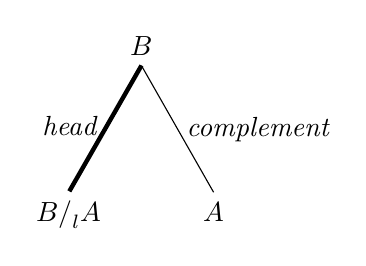
\begin{tikzpicture}[
	level distance=60pt, 
	sibling distance=30pt,
	t/.style={text height=1.5ex, text depth=.25ex, rectangle, outer sep=0pt}, 
	node distance=10pt]
	\Tree [.{$\ty{B}$} \edge[head] node[midway,left,t]{$\textit{head}$}; {$\ty{B}/_l\ty{A}$} \edge node[midway,right,t]{$\textit{complement}$}; {$\ty{A}$} ]
	\end{tikzpicture}
	&
	&
	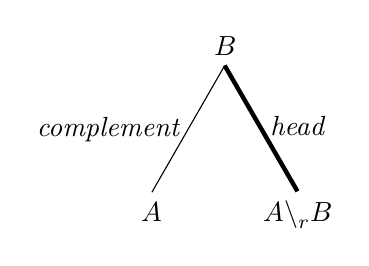
\begin{tikzpicture}[
	level distance=60pt, 
	sibling distance=30pt,
	t/.style={text height=1.5ex, text depth=.25ex, rectangle, outer sep=0pt}, 
	node distance=10pt]
	\Tree [.{$\ty{B}$} \edge node[midway,left,t]{$\textit{complement}$}; {$\ty{A}$} \edge[head] node[midway,right,t]{$\textit{head}$}; {$\ty{A}\bs_r\ty{B}$} ]
	\end{tikzpicture}\\
	\multicolumn{1}{@{}c@{}}{\visible<2>{\alert{$\ty{B /_l A } \equiv \ty{\dbox (B / A)}$\hphantom{lement}}}}
	& &
	\multicolumn{1}{@{}c@{}}{\visible<2>{\alert{\hphantom{lement}$\ty{A \bs_r B } \equiv \ty{\dbox (A \bs  B)}$}}}\\
	\addlinespace\addlinespace\addlinespace
	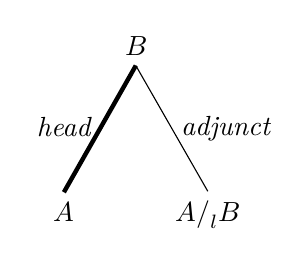
\begin{tikzpicture}[
	level distance=60pt, 
	sibling distance=30pt,
	t/.style={text height=1.5ex, text depth=.25ex, rectangle, outer sep=0pt},
	node distance=10pt]
	\Tree [.{$\ty{B}$} \edge[head] node[midway,left,t]{$\textit{head}$}; {$\ty{A}$} \edge node[midway,right,t]{$\textit{adjunct}$}; {$\ty{A}/_l\ty{B}$} ]
	\end{tikzpicture}
	& &
	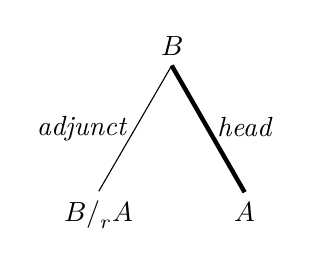
\begin{tikzpicture}[
	level distance=60pt, 
	sibling distance=30pt,
	t/.style={text height=1.5ex, text depth=.25ex, rectangle, outer sep=0pt}, 
	node distance=10pt]
	\Tree [.{$\ty{B}$} \edge node[midway,left,t]{$\textit{adjunct}$}; {$\ty{B}/_r\ty{A}$} \edge[head] node[midway,right,t]{$\textit{head}$}; {$\ty{A}$} ]
	\end{tikzpicture}\hspace{1.3em}\\
	\multicolumn{1}{@{}c@{}}{\visible<2>{\alert{$\ty{A /_l B } \equiv \ty{\ddia A / B}$\hphantom{adjunct}}}}
	& & 
	\multicolumn{1}{@{}c@{}}{\alert{\hphantom{adjunct}\visible<2>{$\ty{B /_r A } \equiv \ty{ B / \ddia A}$}}}\\
	\end{tabularx}\end{center}\vfill
\end{frame}

\begin{frame}{Persistent Modal Structure\smaller\\
\quad\light{A Modern Refinement}}\smaller
	\begin{itemize}
	\item Let $\deps := \complements \mathbin{\cup} \adjuncts$, where:
	\begin{itemize}
		\item \eqmakebox[line][l]{\eqmakebox[ds][l]{$\complements$} $:= \{\su, \obj, \io, \predc, \dots \}$ } \light{-\,- \textit{mandatory complements}}
		\item \eqmakebox[line][l]{\eqmakebox[ds][l]{$\adjuncts$} $:= \{\ddet, \dmod, \dots \}$} \light{-\,- \textit{optional adjuncts}}
	\end{itemize}
	\item Instantiate a residuated pair $(\dxdia[\dep{d}], \dxbox[\dep{d}])$ for each $\dep{d} \in \deps$.
	\item Type grammatical functors as:
	\begin{itemize}
		\item \eqmakebox[line][l]{$\ty{\dxdia[d] A \li B}$} \light{-\,- \textit{head assigning dependency role $\dep{d}$ to its complement $\ty{A}$}}
		\item \eqmakebox[line][l]{$\ty{\dxbox[d] (A \li B)}$} \light{-\,- \textit{adjunct projecting its own role $\dep{d}$}}
	\end{itemize}
	\end{itemize}
\end{frame}

\begin{frame}{Dependency Modalities\smaller\\
\quad\light{Labeled FA Structures}}\smaller
\vspace{1em}
	\colorat{light!30}{2,4}{
	\begin{tabular}{@{}r@{ :: }l@{}}
		\w{the}			& $\ty{\dxbox[\ddet](np/n)}$\\
		\w{culling} 	& $\ty{n}$\\
		\w{necessary} 	& $\ty{\dxbox[\dmod](n/n)}$\\
		\visible<3->{\w{was} 		& $\ty{(\dxdia[\su] np\bs s) / (\dxdia[\predc]\dxbox[\dmod](n / n))}$}
	\end{tabular}}
	\vfill
	
	\alt<3->{
		\colorat{light!30}{4}{
		\[
			\infer[\bs_E]{(\struct[\su]{(\struct[\ddet]{\markproofleaf{n1}{\w{the}}} \sbr \markproofleaf{n2}{\w{culling}})}\cdot(\markproofleaf{n3}{\w{was}} \sbr \struct[\predc]{\markproofleaf{n4}{\w{necessary}}})) \vdash \ty{s}}{
				\infer[\dxdia_I]{\struct[\su]{(\struct[\ddet]{\w{the}} \sbr \w{culling})} \vdash \ty{\dxdia[\su]np}}{
					\infer[/_E]{(\struct[\ddet]{\w{the}} \sbr \w{culling}) \vdash \ty{np}}{
						\infer[\dxbox_E]{\struct[\ddet]{\w{the}} \vdash \ty{np/n}}{
							\infer[\Lex]{\ty{\dxbox[\ddet](np/n)}}{\w{the}}
						}
						&
						\infer[\Lex]{\ty{n}}{\w{culling}}
					}
				}
				&
				\infer[/_E]{(\w{was} \sbr \struct[\predc]{\w{necessary}}) \vdash \ty{\dxdia[\su] np\bs s}}{
					\infer[\Lex]{\ty{(\dxdia[\su] np\bs s) / (\dxdia[\predc]\dxbox[\dmod](n / n))}}{\w{was}}
					&
					\infer[\dxdia_I]{\struct[\predc]{\w{necessary}} \vdash \ty{\dxdia[\predc]\dxbox[\dmod](n / n)}}{
						\infer[\Lex]{\ty{\dxbox[\dmod](n / n)}}{\w{necessary}}
					}
				}
			}
		\]
		}
		\visible<4->{
		\begin{tikzpicture}[remember picture, overlay,
		    every node/.style={
		        inner sep=0pt,
		        minimum height=0pt,
		        text depth=0.3em,
		        align=center,
		        color=pred
		    },
		]
		  \arc{n3}{n4}{-0.45}{\predc}
		  \arc{n3}{n2}{-0.585}{\su}
		  \arc{n2}{n1}{-0.47}{\ddet}
		\end{tikzpicture}
		}
	}{
		\colorat{light!30}{2}{
		\[
			\infer[/_E]{(\struct[\ddet]{\markproofleaf{n1}{\w{the}}} \sbr (\struct[\dmod]{\markproofleaf{n2}{\w{necessary}}} \sbr \markproofleaf{n3}{\w{culling}})) \vdash \ty{np}}{
				\infer[\dxbox_E]{\struct[\ddet]{\w{the}} \vdash \ty{np/n}}{
					\infer[\Lex]{\ty{\dxbox[\ddet](np/n)}}{\w{the}}
				}
				&
				\infer[/_E]{(\struct[\dmod]{\w{necessary}} \sbr \w{culling}) \vdash \ty{n}}{
					\infer[\dxbox_E]{\struct[\dmod]{\w{necessary}} \vdash \ty{n / n}}{
						\infer[\Lex]{\ty{\dxbox[\dmod]n/n}}{\w{necessary}}
					}
					&
					\infer[\Lex]{\ty{n}}{\w{culling}}
				}
			}
		\]
		}
		\visible<2->{
		\begin{tikzpicture}[remember picture, overlay,
		    every node/.style={
		        inner sep=0pt,
		        minimum height=0pt,
		        text depth=0.3em,
		        align=center,
		        color=pred
		    },
		]
		  \arc{n3}{n1}{-1.7}{\ddet}
		  \arc{n3}{n2}{-0.6}{\dmod}
		\end{tikzpicture}
		}
	}
\end{frame}

\begin{frame}{Dependency Modalities\smaller\\
\quad\light{Variations on a Theme}}\smaller
	\begin{itemize}
		\item Dependency domains $\supseteq$ constituency structures?\\
		\light{-\,- a bottleneck of (and argument for) free associativity}
		\visible<2->{
		\item Dependency cued by morphology?\\
		\light{-\,- lexically pre-assigned complements}
		\visible<3->{
		\item Movement-like phenomena limited to certain dependencies?\\
		\light{-\,- dependency-dependent structural rules}
		\visible<4->{
		\item Dependency resolves ambiguity?\\
		\light{-\,- derivational ambiguity $\rightsquigarrow$ lexical ambiguity}
		}}}
	\end{itemize}\vfill

	\alt<4->{
	Dutch embedded clauses are \alert{verb-final}; e.g.	haten :: $\ty{\dxdia[\su]np \bs (\dxdia[\obj]np \bs s)}$
	\vfill
	
	\visible<5->{
	gender-matched relative clauses are \alert{derivationally ambiguous}:
	\begin{center}
		``\textit{mannen die vrouwen haten}'' $\rightsquigarrow$ ``men that hate women'' \ | \ ``men thate women hate''
	\end{center}
	
	consider instead; die :: $\ty{\dxbox[\dmod](n \bs n) / (\dxdia[\obj] np \bs s) \& \dxbox[\dmod](n \bs n) / (\dxdia[\su] np \bs s)}$
	}}{
	\smaller
	\alt<3->{
		\[
			\infer*{}{
				\infer={}{
					\infer=[\rulestyle{top}]{\Gamma\subst{(\struct[\su]{\Delta} \cdot (\struct[\obj]{\Xi} \cdot \Theta)) } \vdash \ty{A}}{
						\Gamma\subst{(\struct[\su]{\Delta} \cdot (\Theta \cdot \struct[\obj]{\Xi}))} \vdash \ty{A}
					}
				}
			}
		\]
		\vfill
		\begin{flushright}
			\light{or perhaps: \EX{} holds within the sentential domain (yet no word salad\dots)}
		\end{flushright}
	}{
	\alt<2->{
		\begin{minipage}{0.3\textwidth}
		\begin{tabular}{@{}r@{ :: }l@{}}
		luin   (\light{read})  		& $\ty{(\dxdia[\su]np \bs s) / \dxdia[\obj] np}$ \\ 
		min\"a (\light{I-nom}) 		& $\ty{\alert{\dxbox[\su]}\dxdia[\su]np}$ \\
		kirjan (\light{book-acc}) 	& $\ty{\alert{\dxbox[\obj]}\dxdia[\obj]np}$
		\end{tabular}		
		\end{minipage}\hfil
		\begin{minipage}{0.5\textwidth}
		\centering
		$
			\infer[\bs_E]{\struct[\su]{\w{min\"a}} \cdot \w{luin} \cdot \struct[\obj]{\w{kirjan}} \vdash \ty{s}}{
				\infer[\dxbox_E]{\struct[\su]{\w{min\"a}} \vdash \ty{\dxdia[\su]np}}{
					\infer[\Lex]{\ty{\dxbox[\su]\dxdia[\su]np}}{\w{min\"a}}
				}
				&
				\infer[/_E]{\w{luin} \cdot \struct[\obj]{\w{kirjan}} \vdash \ty{\dxdia[\su]np \bs s}}{
					\infer[\Lex]{\ty{(\dxdia[\su]np \bs s) / \dxdia[\obj] np}}{\w{luin}}
					&
					\infer[\dxbox_E]{\struct[\obj]{\w{kirjan}} \vdash \ty{\dxdia[\obj]np}}{
						\infer[\Lex]{\ty{\dxbox[\obj]\dxdia[\obj]np}}{\w{kirjan}}
					}
				}
			}
		$
		\end{minipage}
	}{
		\[
			(\struct[\su]{(\struct[\ddet]{\w{the}} \sbr \w{culling})}\cdot(\w{was} \sbr \struct[\predc]{\w{necessary}}))
			\mathbin{\alert{\rightsquigarrow}}
			\struct[\su]{\struct[\ddet]{\w{the}} \sbr \w{culling}}\cdot \w{was} \sbr \struct[\predc]{\w{necessary}}
		\]
	}}}
\end{frame}


\begin{frame}{Nameless\smaller\\
\quad\light{Horizontal Movement}}\smaller
	\alt<2->{
		\[
		\infer*{
			((\struct[\ddet]{\markproofleaf{n1}{\w{the}}} \cdot \markproofleaf{n2}{\w{violence}}) \cdot \struct[\dmod]{(\markproofleaf{n3}{\w{that}} \cdot \struct[\body]{(\struct[\su]{(\struct[\ddet]{\markproofleaf{n4}{\w{the}}} \cdot \markproofleaf{n5}{\w{world}})} \cdot (\markproofleaf{n6}{\w{ignores}} \cdot \struct[\dmod]{\markproofleaf{n7}{\w{happily}}}))})})
		}{}
		\]
		\begin{tikzpicture}[remember picture, overlay]
			\arc{n2}{n1}{-0.5}{\ddet}
			\arc{n2}{n3}{-0.5}{\dmod}
			\arc{n3}{n6}{-1.5}{\body}
			\arc{n6}{n5}{-0.5}{\su}
			\arc{n5}{n4}{-0.5}{\ddet}
			\arc{n6}{n7}{-0.5}{\dmod}
		\end{tikzpicture}
	}{
	that :: \sout{$\ty{(n \bs n) / (s / np )}$} \ \sout{$\ty{(n \bs n) / (s / \ddia\dbox np )}$} $\ty{(\dxbox[\dmod](n \bs n) / \dxdia[\body](s / \alert{\ddia\dbox}\dxdia[\obj] np))}$
	\vfill
	\smaller
	$	\hspace{-1em}
		\infer[\dxbox_E]{\struct[\dmod]{(\w{that} \cdot \struct[\body]{(\struct[\su]{(\struct[\ddet]{\w{the}} \cdot \w{world})} \cdot (\w{ignores} \cdot \struct[\dmod]{\w{happily}}))})} \vdash n \bs n}{
			\infer[/_E]{(\w{that} \cdot \struct[\body]{(\struct[\su]{(\struct[\ddet]{\w{the}} \cdot \w{world})} \cdot (\w{ignores} \cdot \struct[\dmod]{\w{happily}}))}) \vdash \ty{\dxbox[\dmod](n \bs n)}}{
				\infer[\Lex]{\dots\vphantom{\dxdia[\su]}}{\w{that}} 
%				\ty{(\dxbox[\dmod](n \bs n) / \dxdia[\body](s / \ddia\dbox\dxdia[\obj] np))}}
				&
				\hspace{-3.8em}
				\infer[\dxdia_I]{\struct[\body]{(\struct[\su]{(\struct[\ddet]{\w{the}} \cdot \w{world})} \cdot (\w{ignores} \cdot \struct[\dmod]{\w{happily}}))} \vdash \ty{\dxdia[\body](s / \ddia \dbox\dxdia[\obj] np)}}{
					\infer[/_I]{(\struct[\su]{(\struct[\ddet]{\w{the}} \cdot \w{world})} \cdot (\w{ignores} \cdot \struct[\dmod]{\w{happily}})) \vdash \ty{s / \ddia \dbox\dxdia[\obj] np}}{
						\infer[\ddia_E]{((\struct[\su]{(\struct[\ddet]{\w{the}} \cdot \w{world})} \cdot (\w{ignores} \cdot \struct[\dmod]{\w{happily}}))\cdot\ty{\ddia\dbox\dxdia[\obj]np}) \vdash \ty{s}}{
							\infer[\Ax]{\ty{\ddia\dbox\dxdia[\obj] np} \vdash \ty{\ddia\dbox\dxdia[\obj] np}}{}
							&
							\hspace{-8em}
							\infer[A^r_{\ddia}]{((\struct[\su]{(\struct[\ddet]{\w{the}} \cdot \w{world})} \cdot (\w{ignores} \cdot \struct[\dmod]{\w{happily}}))\cdot\struct{\ty{\dbox\dxdia[\obj] np}}) \vdash \ty{s}}{
								\infer[C^r_{\ddia}]{(\struct[\su]{(\struct[\ddet]{\w{the}} \cdot \w{world})} \cdot ((\w{ignores} \cdot \struct[\dmod]{\w{happily}})\cdot\struct{\ty{\dbox\dxdia[\obj] np}})) \vdash \ty{s}}{
									\infer[\bs_E]{(\struct[\su]{(\struct[\ddet]{\w{the}} \cdot \w{world})} \cdot ((\w{ignores} \cdot \struct{\ty{\dbox\dxdia[\obj] np}})\cdot\struct[\dmod]{\w{happily}}))  \vdash \ty{s}}{
										\infer[\dxdia_I]{\struct[\su]{(\struct[\ddet]{\w{the}} \cdot \w{world})} \vdash \ty{\dxdia[\su]np}}{
											\hspace{-4em}
											\infer[/_E]{(\struct[\ddet]{\w{the}} \cdot \w{world}) \vdash \ty{np}}{
													\infer[\dxbox_E]{\struct[\ddet]{\w{the}} \vdash \ty{np / n}}{
														\infer[\Lex]{\ty{\dxbox[\ddet](np/n)}}{\w{the}}
													}
													&
													\infer[\Lex]{\ty{n}}{\w{world}}
											}
										}
										&
%										\hspace{-3em}
										\infer[\bs_E]{((\w{ignores} \cdot \struct{\ty{\dbox\dxdia[\obj] np}})\cdot\struct[\dmod]{\w{happily}}) \vdash \ty{\dxdia[\su]np \bs s}}{
											\infer[/_E]{(\w{ignores} \cdot \struct{\ty{\dbox\dxdia[\obj] np}}) \vdash \ty{\dxdia[\su]np \bs s}}{
												\infer[\Lex]{\ty{(\dxdia[\su] np \bs s)/\dxdia[\obj] np}}{\w{ignores}}
												&
												\infer[\dbox_E]{\struct{\ty{\dbox\dxdia[\obj] np}} \vdash \dxdia[\obj]\ty{np}}{
													\infer[\Ax]{\ty{\dbox\dxdia[\obj] np} \vdash \ty{\dbox \dxdia[\obj]np}}{}
												}
											}
											&
											\hspace{-0.5em}
											\infer[\dxbox_E]{\struct[\dmod]{\w{happily}} \vdash (\dxdia[\su]np\bs s)\bs \dxdia[\su]np\bs s}{
												\infer[\Lex]{\ty{\dxbox[\dmod]((\dxdia[\su]np\bs s)\bs \dxdia[\su]np\bs s)}}{\w{happily}}
											}
										}
									}
								}
							}
						}
					}
				}
			}
		}
	$
	}
\end{frame}

\begin{frame}{Dependency Modalities\smaller\\
\quad\light{Vertical Movement}}\smaller
\end{frame}

\begin{frame}{TLDR}

\end{frame}


\end{document}